\documentclass{article}\usepackage[]{graphicx}\usepackage[]{color}
%% maxwidth is the original width if it is less than linewidth
%% otherwise use linewidth (to make sure the graphics do not exceed the margin)
\makeatletter
\def\maxwidth{ %
  \ifdim\Gin@nat@width>\linewidth
    \linewidth
  \else
    \Gin@nat@width
  \fi
}
\makeatother

\definecolor{fgcolor}{rgb}{0.345, 0.345, 0.345}
\newcommand{\hlnum}[1]{\textcolor[rgb]{0.686,0.059,0.569}{#1}}%
\newcommand{\hlstr}[1]{\textcolor[rgb]{0.192,0.494,0.8}{#1}}%
\newcommand{\hlcom}[1]{\textcolor[rgb]{0.678,0.584,0.686}{\textit{#1}}}%
\newcommand{\hlopt}[1]{\textcolor[rgb]{0,0,0}{#1}}%
\newcommand{\hlstd}[1]{\textcolor[rgb]{0.345,0.345,0.345}{#1}}%
\newcommand{\hlkwa}[1]{\textcolor[rgb]{0.161,0.373,0.58}{\textbf{#1}}}%
\newcommand{\hlkwb}[1]{\textcolor[rgb]{0.69,0.353,0.396}{#1}}%
\newcommand{\hlkwc}[1]{\textcolor[rgb]{0.333,0.667,0.333}{#1}}%
\newcommand{\hlkwd}[1]{\textcolor[rgb]{0.737,0.353,0.396}{\textbf{#1}}}%

\usepackage{framed}
\makeatletter
\newenvironment{kframe}{%
 \def\at@end@of@kframe{}%
 \ifinner\ifhmode%
  \def\at@end@of@kframe{\end{minipage}}%
  \begin{minipage}{\columnwidth}%
 \fi\fi%
 \def\FrameCommand##1{\hskip\@totalleftmargin \hskip-\fboxsep
 \colorbox{shadecolor}{##1}\hskip-\fboxsep
     % There is no \\@totalrightmargin, so:
     \hskip-\linewidth \hskip-\@totalleftmargin \hskip\columnwidth}%
 \MakeFramed {\advance\hsize-\width
   \@totalleftmargin\z@ \linewidth\hsize
   \@setminipage}}%
 {\par\unskip\endMakeFramed%
 \at@end@of@kframe}
\makeatother

\definecolor{shadecolor}{rgb}{.97, .97, .97}
\definecolor{messagecolor}{rgb}{0, 0, 0}
\definecolor{warningcolor}{rgb}{1, 0, 1}
\definecolor{errorcolor}{rgb}{1, 0, 0}
\newenvironment{knitrout}{}{} % an empty environment to be redefined in TeX

\usepackage{alltt}
\usepackage{amscd, amssymb, amsmath, verbatim, setspace}
\usepackage[left=1.0in, right=1.0in, top=1.0in, bottom=1.0in]{geometry}
\usepackage{mathrsfs}
\usepackage{listings}


\IfFileExists{upquote.sty}{\usepackage{upquote}}{}
\begin{document}
\begin{flushright}
Arif Ali\\
Math 611 Stochastic Simulation\\
Sept 8, 2016\\
\end{flushright}

\begin{center}
\LARGE\textbf{Homework 1}
  \end{center}
\section*{Exercise 1}
It is given that $U \sim Unif(0,1)$ and that $c>0$

Let $X = g(u) = -c*ln(u) \implies -x/c=ln(u) \implies e^{-x/c}=u$

$\therefore g^{-1}(u) = e^{-u/c}$

$X = \int^{x}_{0}e^{-x/c}=-\frac{1}{c}e^{-x/c}+\frac{1}{c}$

$dX/dx = 1/c*e^{-x/c} \sim exp(1/c)$

\section*{Exercise 2}

\section*{Exercise 3}
\subsection*{Part A}

Let $z = 1+e^{-(x-\mu)/\beta} \implies dz = -\frac{1}{\beta}e^{-(x-\mu)/\beta}*dx \implies dx = \frac{dz}{-\frac{1}{\beta}e^{-(x-\mu)/\beta}}$
\begin{equation}
F(x) = \int^{x}_{-\infty} f(x) dx = \int\frac{1}{\beta}\frac{e^{-(x-\mu)/\beta}}{(1+e^{-(x-\mu)/\beta})^2}dx=
\int\frac{1}{\beta}\frac{e^{-(x-\mu)/\beta}}{z^2}*\frac{dz}{-\frac{1}{\beta}e^{-(x-\mu)/\beta}}=
\int-\frac{1}{z^2}dz=\\
\frac{1}{z}=\big|^{x}_{-\infty}\frac{1}{1+e^{-(x-\mu)/\beta}}=\frac{1}{1+e^{-(x-\mu)/\beta}}
\end{equation}

To find the inverse, we do the following

$Y = \frac{1}{1+e^{-(x-\mu)/\beta}} \implies\\
1+e^{-(x-\mu)/\beta} = \frac{1}{Y} \implies\\
e^{-(x-\mu)/\beta} = \frac{1}{Y} - 1 \implies\\
-(x-\mu)/\beta = ln(\frac{1}{Y} - 1) \implies\\
-(x-\mu) = ln(\frac{1}{Y} - 1)\beta \implies\\
x = \mu - ln(\frac{1}{Y} - 1)\beta$
\begin{knitrout}
\definecolor{shadecolor}{rgb}{0.969, 0.969, 0.969}\color{fgcolor}\begin{kframe}
\begin{alltt}
\hlstd{u} \hlkwb{=} \hlkwd{runif}\hlstd{(}\hlnum{1e4}\hlstd{)}

\hlstd{inverse_logistic_cdf} \hlkwb{=} \hlkwa{function}\hlstd{(}\hlkwc{x}\hlstd{,} \hlkwc{mu} \hlstd{=} \hlnum{0} \hlstd{,} \hlkwc{B} \hlstd{=} \hlnum{1}\hlstd{)\{}
  \hlstd{mu} \hlopt{-} \hlkwd{log}\hlstd{(}\hlnum{1}\hlopt{/}\hlstd{x}\hlopt{-}\hlnum{1}\hlstd{)}\hlopt{*}\hlstd{B}
\hlstd{\}}

\hlstd{it_logistic} \hlkwb{=} \hlkwd{inverse_logistic_cdf}\hlstd{(u)}
\hlstd{r_logistic} \hlkwb{=} \hlkwd{rlogis}\hlstd{(}\hlnum{1e4}\hlstd{)}

\hlkwd{hist}\hlstd{(it_logistic,} \hlkwc{breaks} \hlstd{=} \hlnum{50}\hlstd{,} \hlkwc{col} \hlstd{=} \hlstr{"green"}\hlstd{)}
\hlkwd{hist}\hlstd{(r_logistic,} \hlkwc{breaks} \hlstd{=} \hlnum{50}\hlstd{,} \hlkwc{col} \hlstd{=} \hlstr{"#FF000099"}\hlstd{,} \hlkwc{add} \hlstd{= T)}
\end{alltt}
\end{kframe}
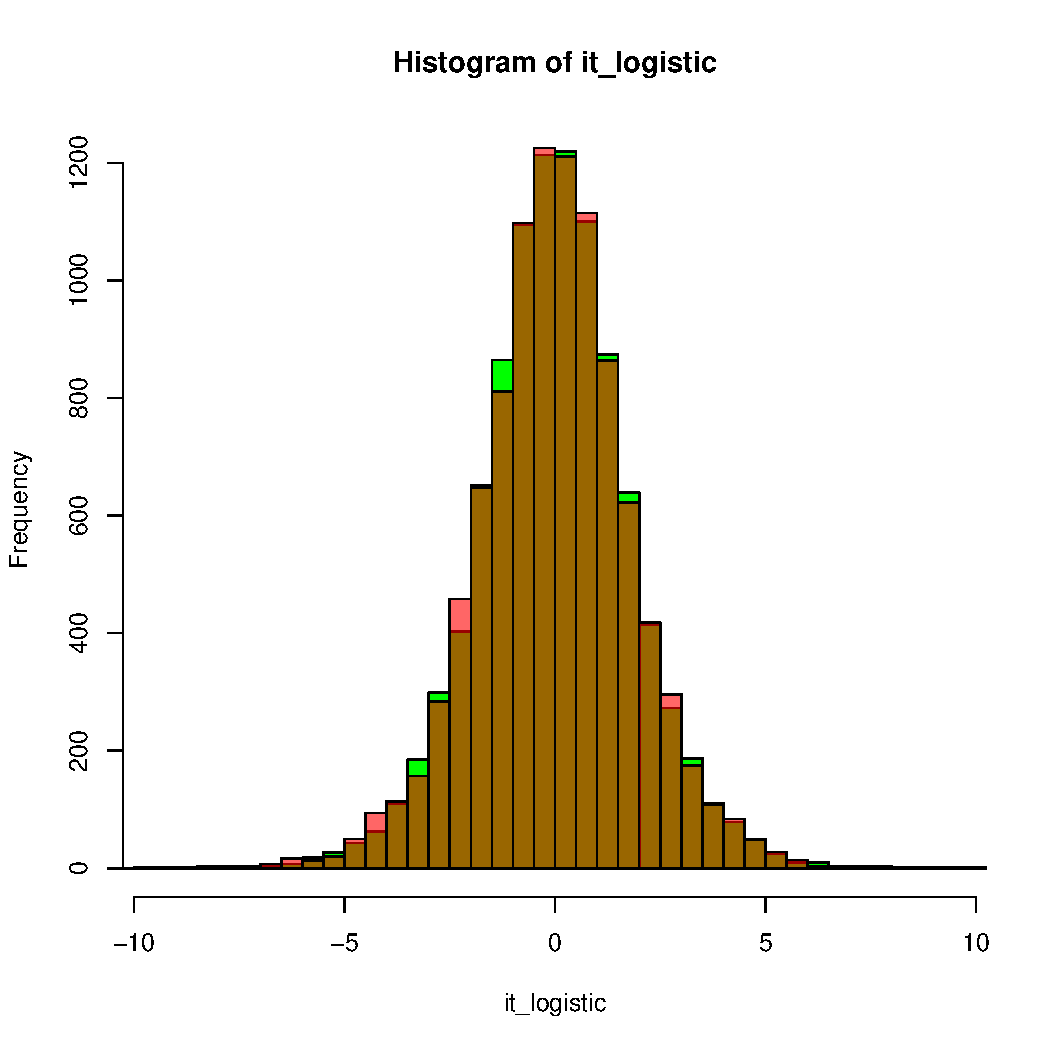
\includegraphics[width=0.50\linewidth]{figure/unnamed-chunk-2-1} 

\end{knitrout}

\subsection*{Part B}
\begin{knitrout}
\definecolor{shadecolor}{rgb}{0.969, 0.969, 0.969}\color{fgcolor}\begin{kframe}
\begin{alltt}
\hlstd{inverse_cauchy_cdf} \hlkwb{=} \hlkwa{function}\hlstd{(}\hlkwc{x}\hlstd{,} \hlkwc{mu} \hlstd{=} \hlnum{0}\hlstd{,} \hlkwc{sigma} \hlstd{=} \hlnum{1}\hlstd{)\{}
  \hlstd{sigma}\hlopt{*}\hlkwd{tan}\hlstd{(pi}\hlopt{*}\hlstd{(x}\hlopt{-}\hlnum{0.5}\hlstd{))} \hlopt{+} \hlstd{mu}
\hlstd{\}}

\hlstd{it_cauchy} \hlkwb{=} \hlkwd{inverse_cauchy_cdf}\hlstd{(u)}
\hlstd{r_cauchy} \hlkwb{=} \hlkwd{rcauchy}\hlstd{(}\hlnum{1e4}\hlstd{)}

\hlstd{u} \hlkwb{=} \hlkwd{runif}\hlstd{(}\hlnum{1e4}\hlstd{)}
\hlkwd{hist}\hlstd{(it_cauchy,} \hlkwc{breaks} \hlstd{=} \hlnum{50}\hlstd{,} \hlkwc{col} \hlstd{=} \hlstr{"blue"}\hlstd{)}
\hlkwd{hist}\hlstd{(r_cauchy,} \hlkwc{breaks} \hlstd{=} \hlnum{50}\hlstd{,} \hlkwc{col} \hlstd{=} \hlstr{"#FF000099"}\hlstd{,} \hlkwc{add} \hlstd{= T)}
\end{alltt}
\end{kframe}
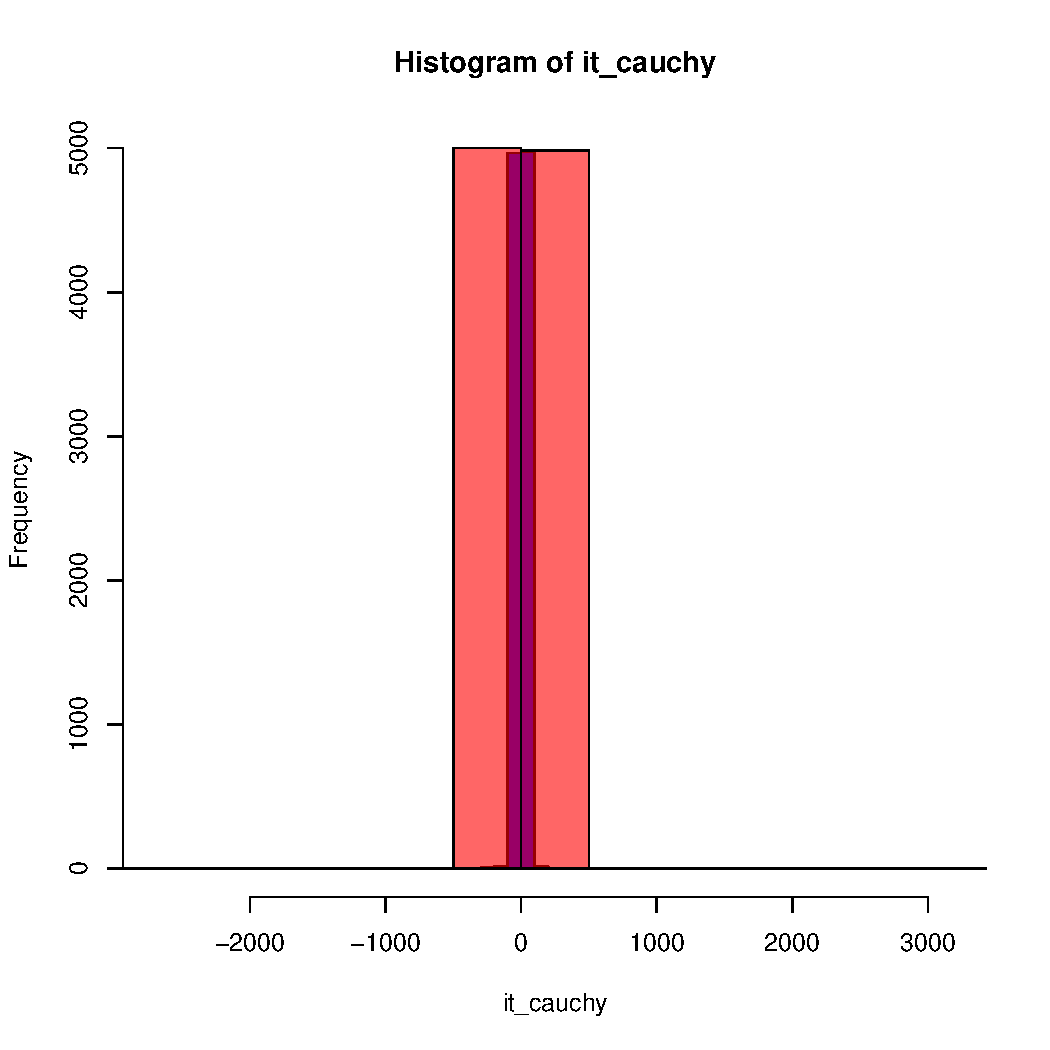
\includegraphics[width=0.50\linewidth]{figure/unnamed-chunk-3-1} 

\end{knitrout}

\section*{Exercise 4}
\begin{knitrout}
\definecolor{shadecolor}{rgb}{0.969, 0.969, 0.969}\color{fgcolor}\begin{kframe}
\begin{alltt}
\hlstd{u1} \hlkwb{=} \hlkwd{runif}\hlstd{(}\hlnum{1e3}\hlstd{)}
\hlstd{u2} \hlkwb{=} \hlkwd{runif}\hlstd{(}\hlnum{1e3}\hlstd{)}

\hlstd{z1} \hlkwb{=} \hlkwd{sqrt}\hlstd{(}\hlopt{-}\hlnum{2}\hlopt{*}\hlkwd{log}\hlstd{(u1))}\hlopt{*}\hlkwd{cos}\hlstd{(}\hlnum{2}\hlopt{*}\hlstd{pi}\hlopt{*}\hlstd{u2)}
\hlstd{z2} \hlkwb{=} \hlkwd{sqrt}\hlstd{(}\hlopt{-}\hlnum{2}\hlopt{*}\hlkwd{log}\hlstd{(u1))}\hlopt{*}\hlkwd{sin}\hlstd{(}\hlnum{2}\hlopt{*}\hlstd{pi}\hlopt{*}\hlstd{u2)}
\hlkwd{qqnorm}\hlstd{(z1)}
\end{alltt}
\end{kframe}
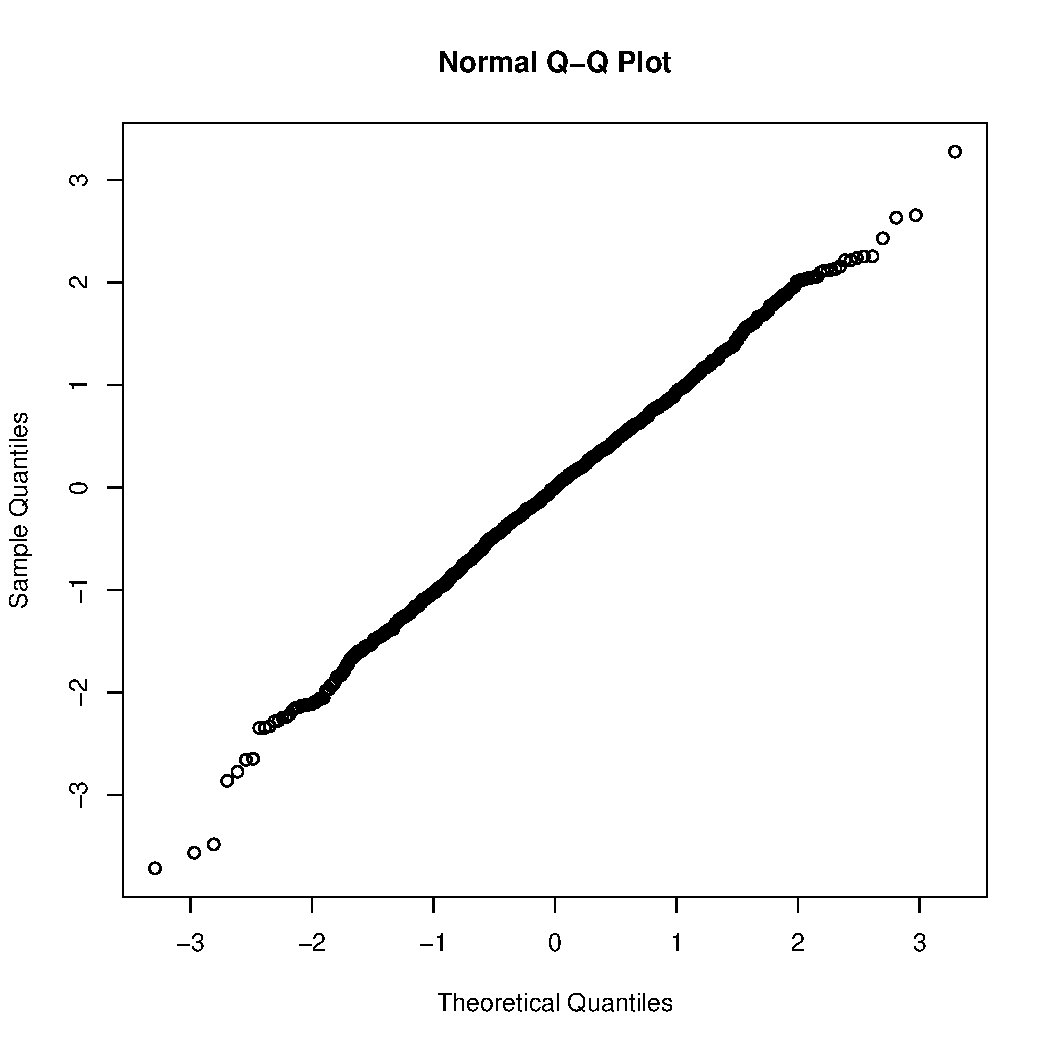
\includegraphics[width=0.50\linewidth]{figure/unnamed-chunk-4-1} 
\begin{kframe}\begin{alltt}
\hlkwd{qqnorm}\hlstd{(z2)}
\end{alltt}
\end{kframe}
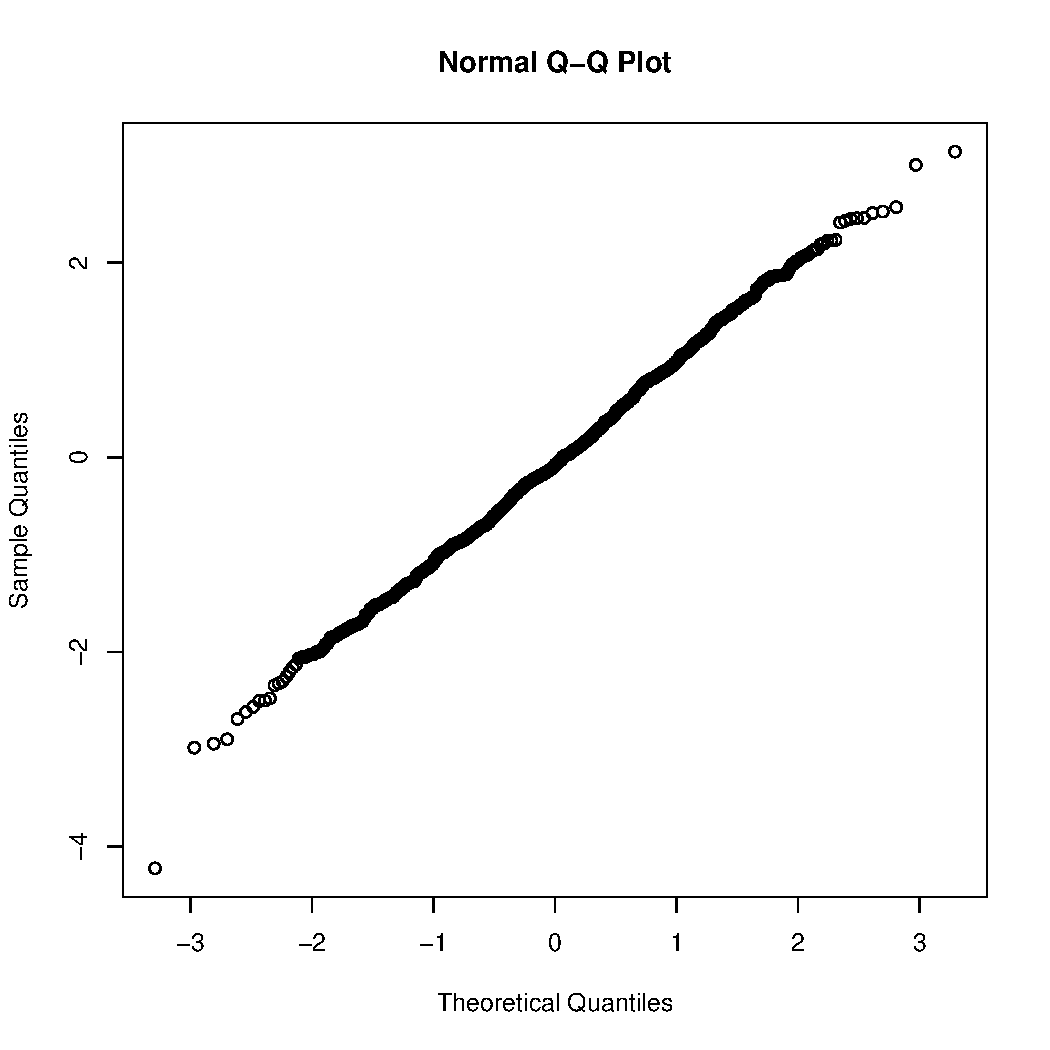
\includegraphics[width=0.50\linewidth]{figure/unnamed-chunk-4-2} 
\begin{kframe}\begin{alltt}
\hlkwd{hist}\hlstd{(z1,} \hlkwc{breaks} \hlstd{=} \hlnum{50}\hlstd{)}
\end{alltt}
\end{kframe}
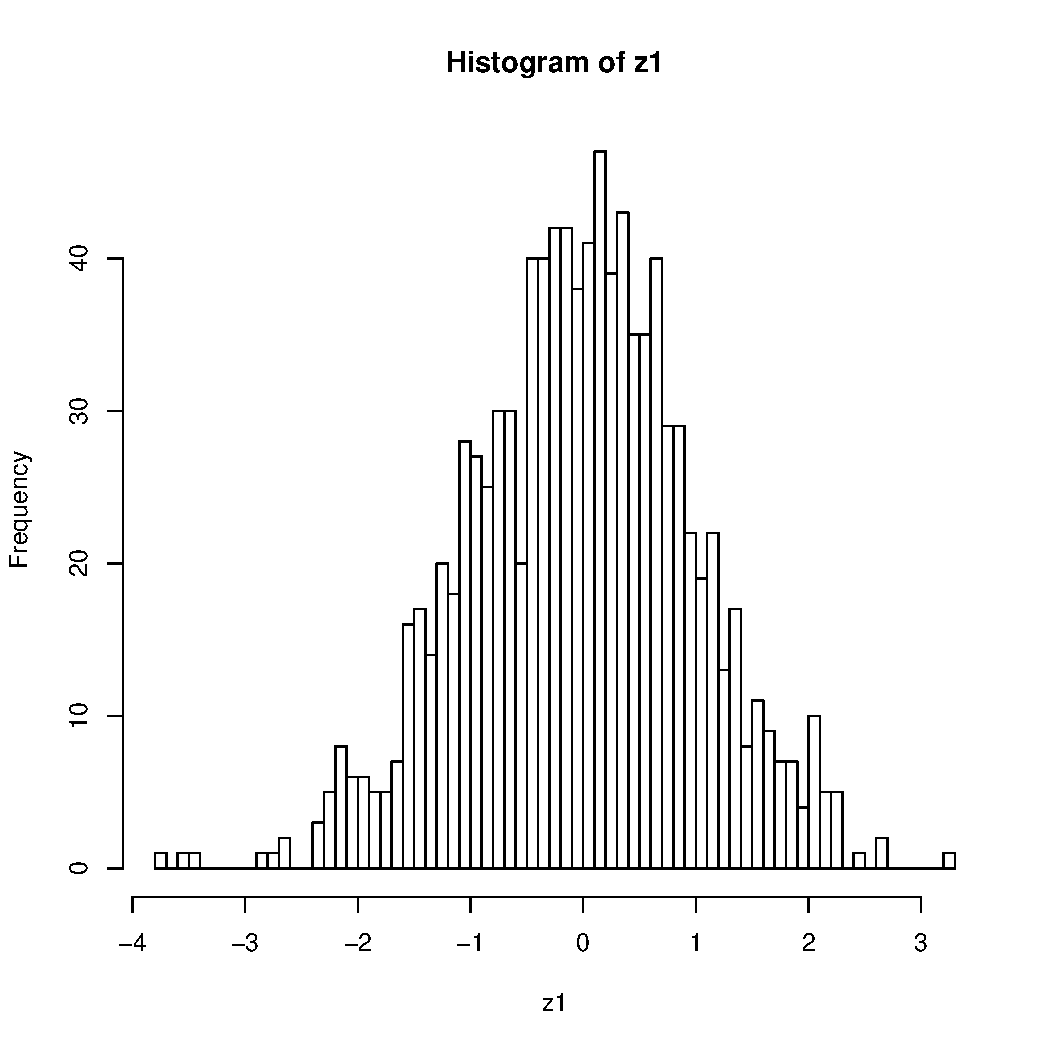
\includegraphics[width=0.50\linewidth]{figure/unnamed-chunk-4-3} 
\begin{kframe}\begin{alltt}
\hlkwd{hist}\hlstd{(z2,} \hlkwc{breaks} \hlstd{=} \hlnum{50}\hlstd{)}
\end{alltt}
\end{kframe}
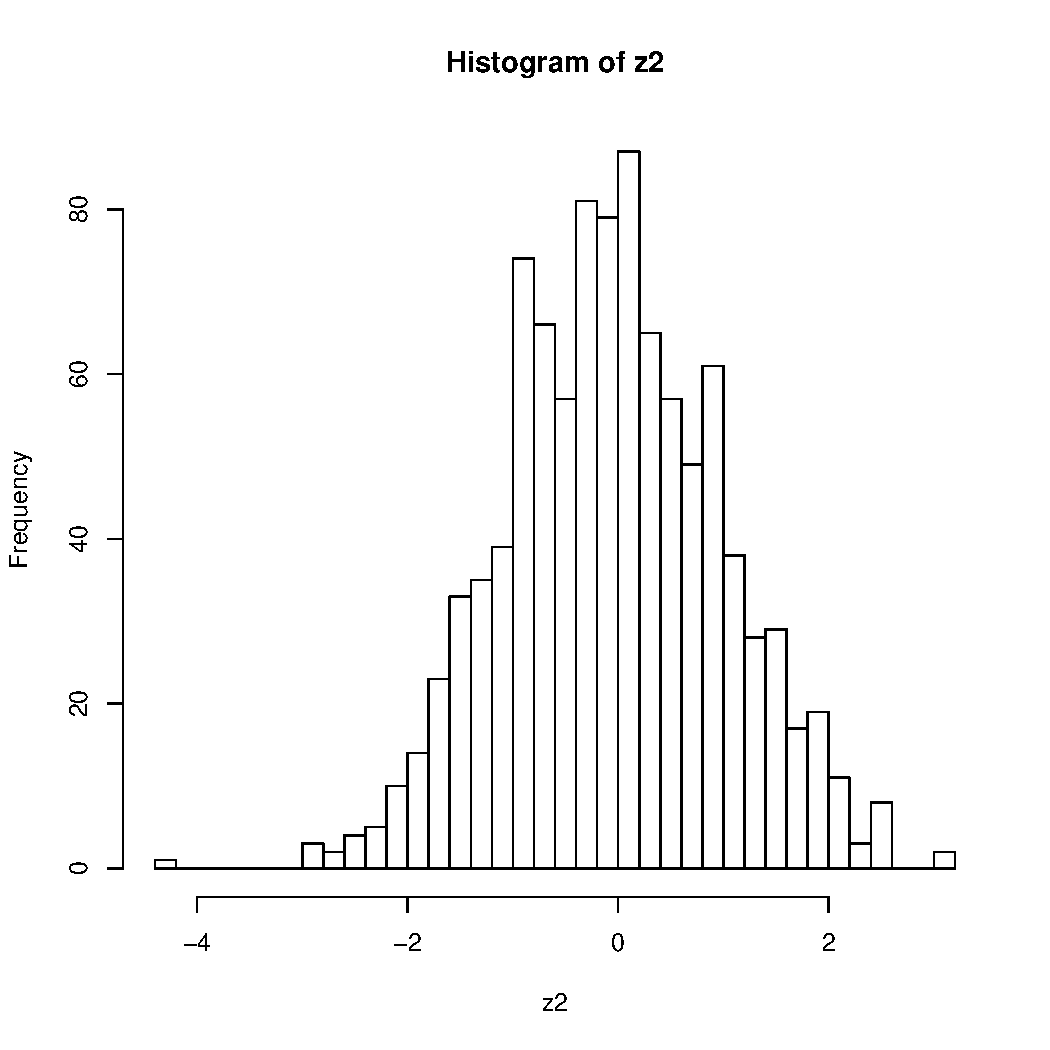
\includegraphics[width=0.50\linewidth]{figure/unnamed-chunk-4-4} 

\end{knitrout}

\section*{Exercise 5}

\end{document}
